\documentclass[12pt, a4paper]{article}

% Document setup
\usepackage[english]{babel}
\usepackage[margin=2.5cm]{geometry}

% Graphics
\usepackage{float}
\usepackage{graphicx}
\graphicspath{ {../figures/} }

% Tables
\usepackage{booktabs}
\usepackage{tabularx}

% Math
\usepackage{amsmath, amsthm}

% Referencing
\usepackage[nameinlink]{cleveref}


% Hypotheses setup
\theoremstyle{remark}
\newtheorem*{nullhypothesis}{Null Hypothesis ($H_0$)}
\newtheorem*{alternativehypothesis}{Alternative Hypothesis ($H_A$)}


\begin{document}

\section{Experiment Design and Setup}

\begin{figure}[H]
	\centering
	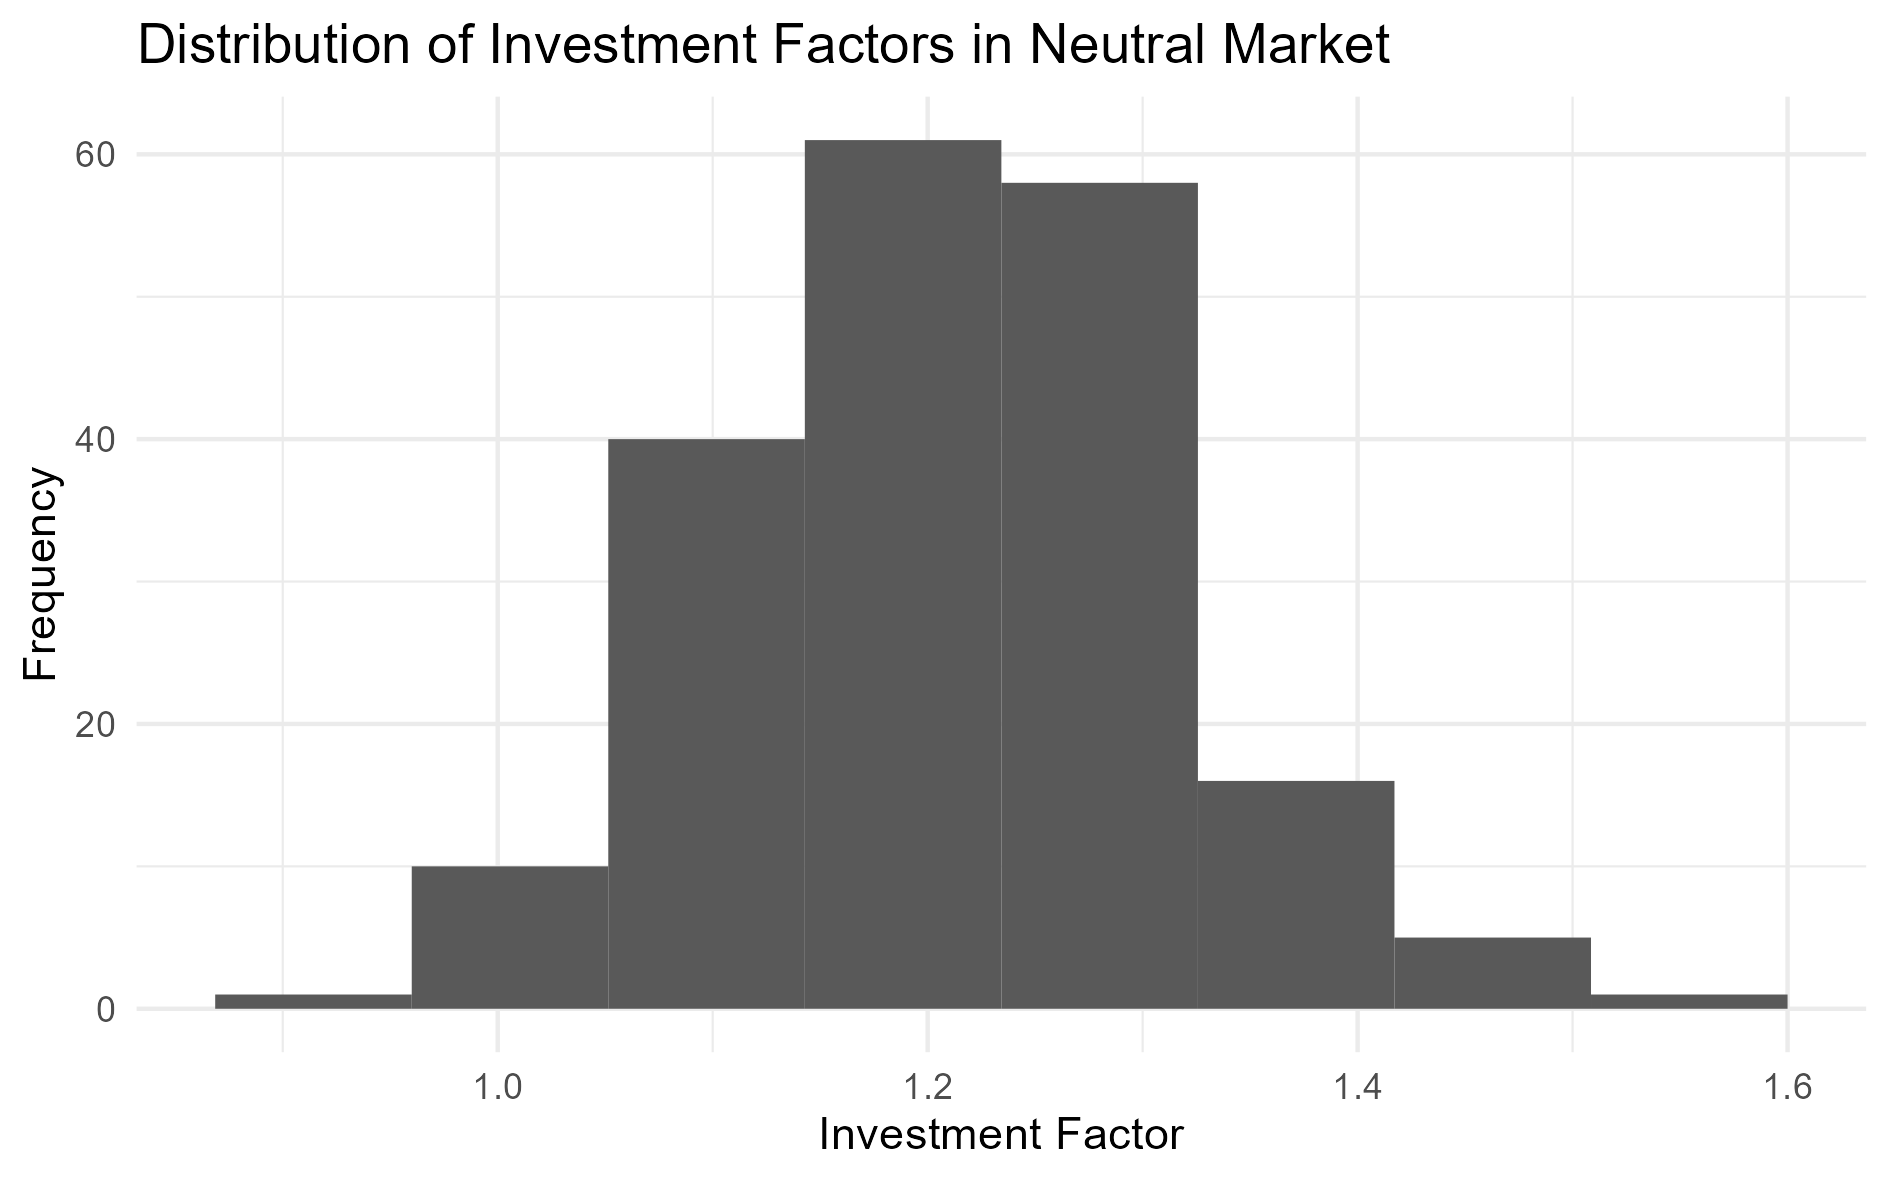
\includegraphics[width=0.7\textwidth]{investment-factors-neutral-market-distribution}
\end{figure}

\begin{figure}[H]
	\centering
	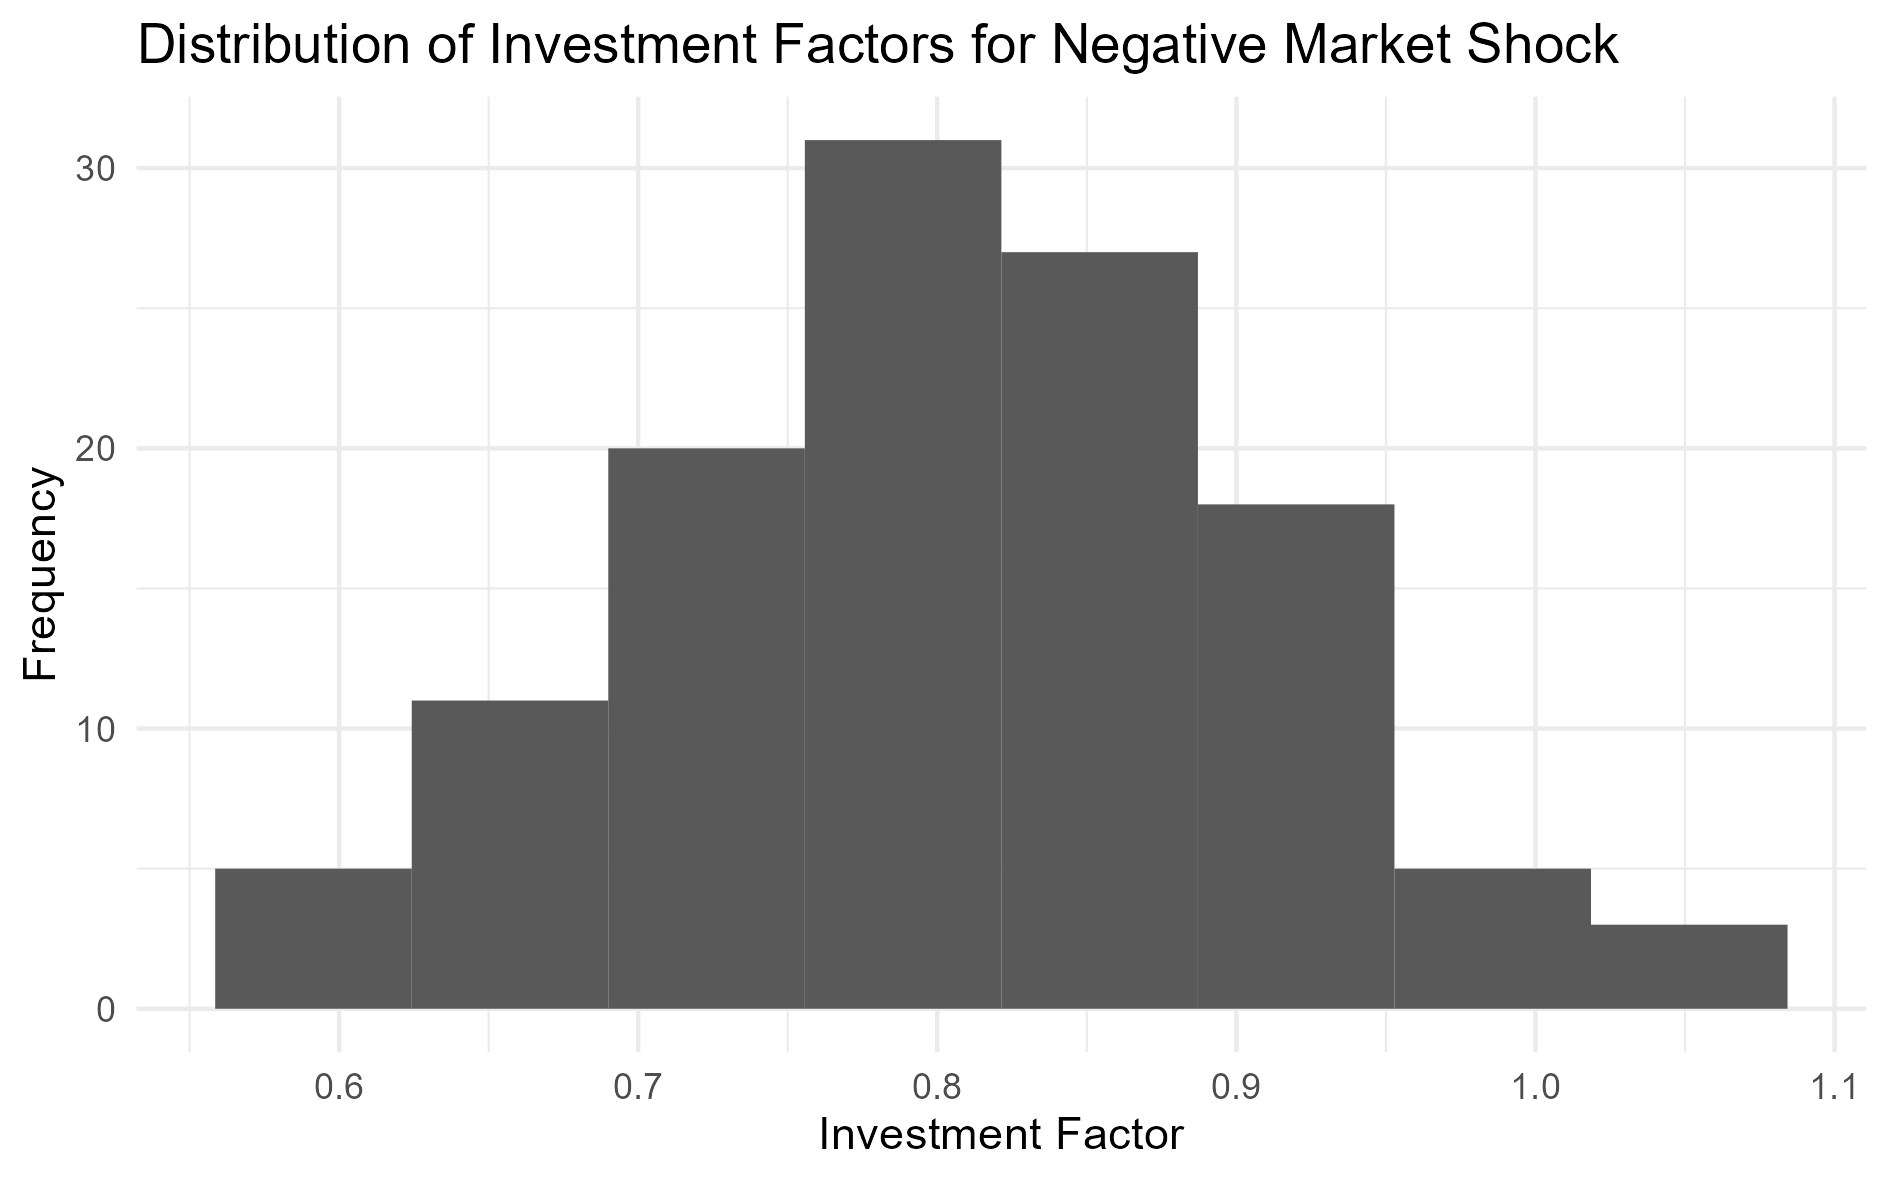
\includegraphics[width=0.7\textwidth]{investment-factors-negative-shock-distribution}
\end{figure}

\begin{figure}[H]
	\centering
	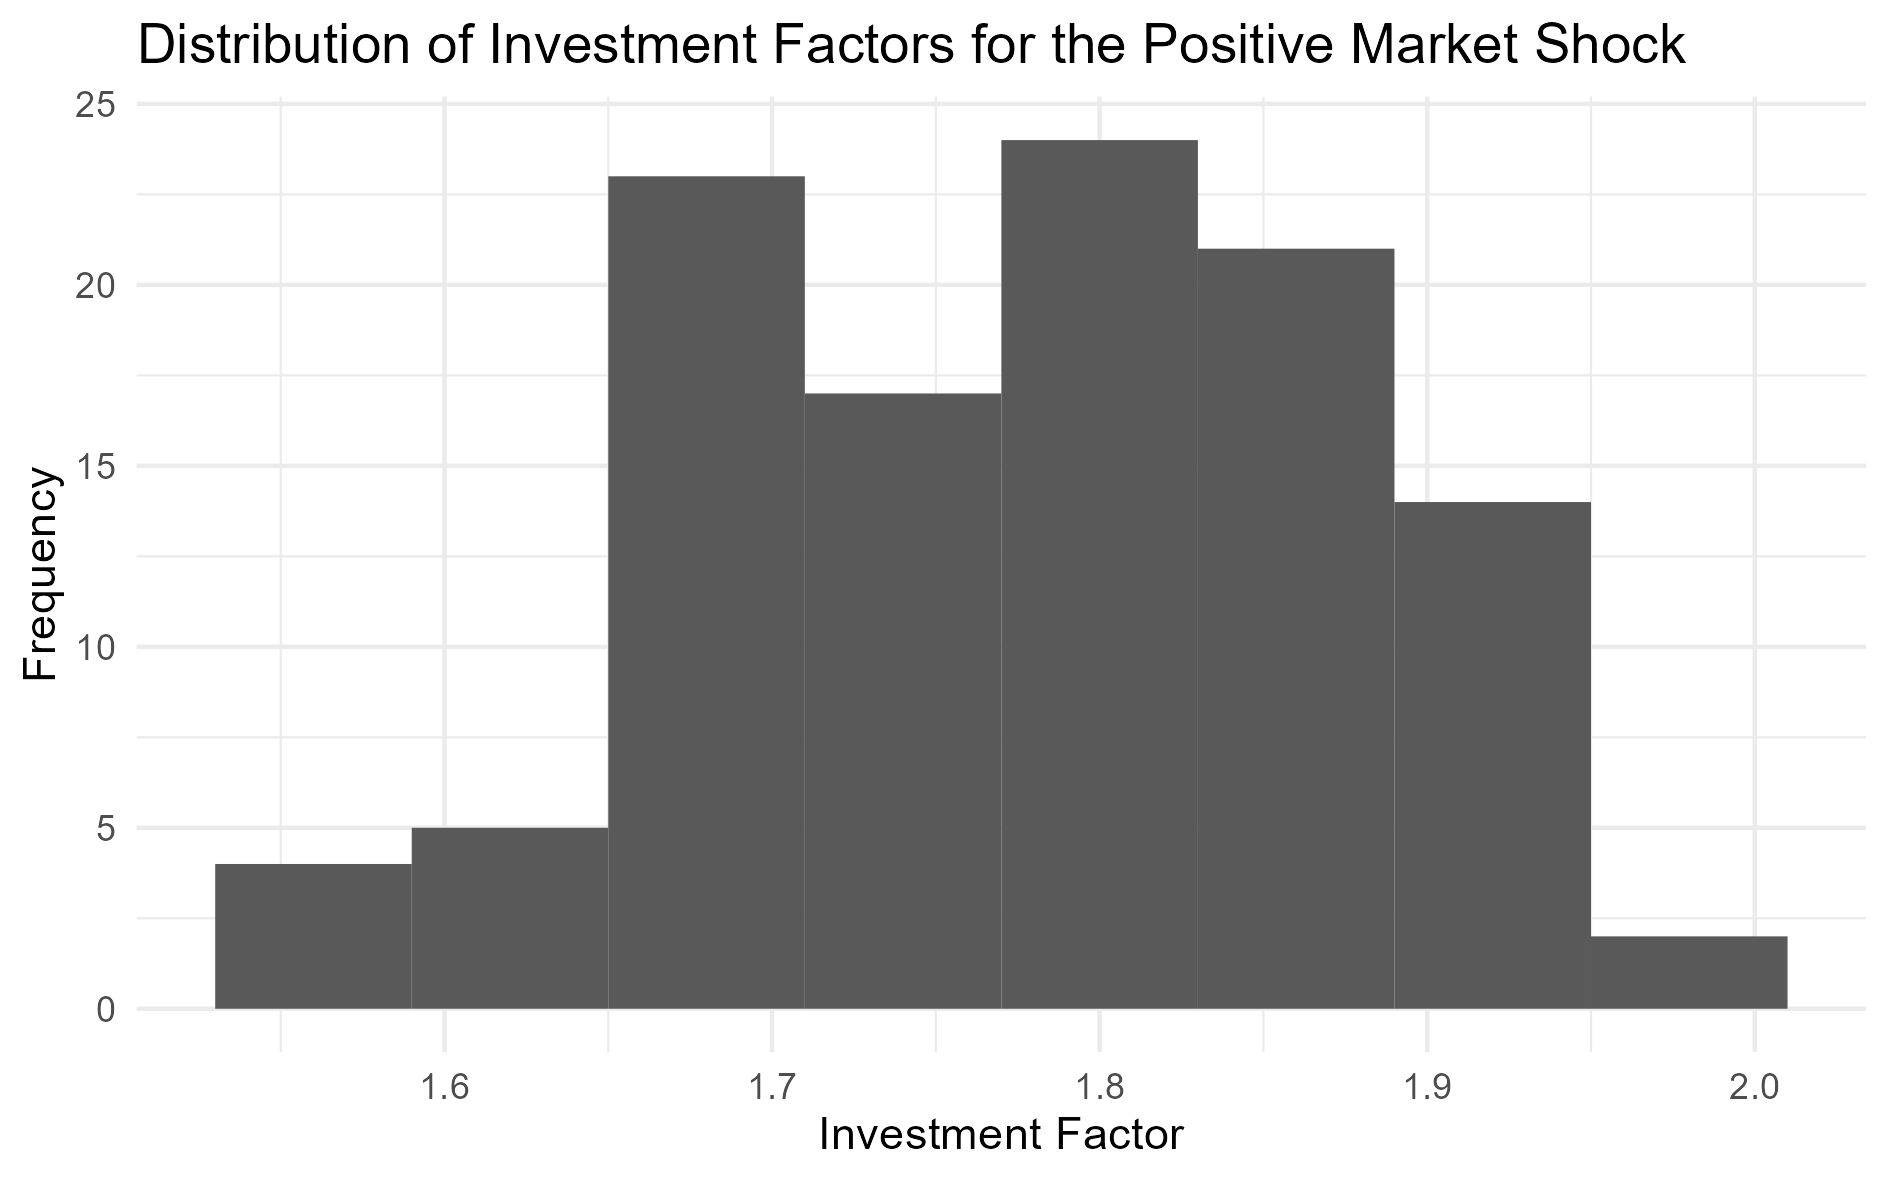
\includegraphics[width=0.7\textwidth]{investment-factors-positive-shock-distribution}
\end{figure}


\section{Aggregate Statistics}

\begin{table}[ht]
\centering
\caption{Investments Summary Statistics (30 Observations)} 
\label{table:InvestmentsSummaryStats}
\begin{tabularx}{\textwidth}{Xrrrr}
  \toprule
Variable & Mean & SD & Min & Max \\ 
  \midrule
Investment Decision Week 4 & 8.700 & 1.968 & 4 & 10 \\ 
  Investment Decision Week 8, Negative Shock Market & 7.533 & 3.889 & 0 & 10 \\ 
  Investment Decision Week 8, Positive Shock Market & 7.190 & 4.174 & 0 & 10 \\ 
  Investment Decision Deviation, Negative Shock Market & -1.467 & 3.583 & -10 & 3 \\ 
  Investment Decision Deviation, Positive Shock Market & -1.210 & 4.066 & -10 & 5 \\ 
   \bottomrule
\end{tabularx}
\end{table}


30 observations in the sample of which half (15) were exposed to a negative and the other half (15) exposed to a positive shock.

At the end of week 4, individuals invested on average 8.7 euros out of their 10 euros. At the end of week 8, individuals who experienced a negative market shock invested on average 7.53 euros and individuals who experienced a positive marketed shock invested 7.19 out of their 10 euros.

\begin{figure}[H]
	\centering
	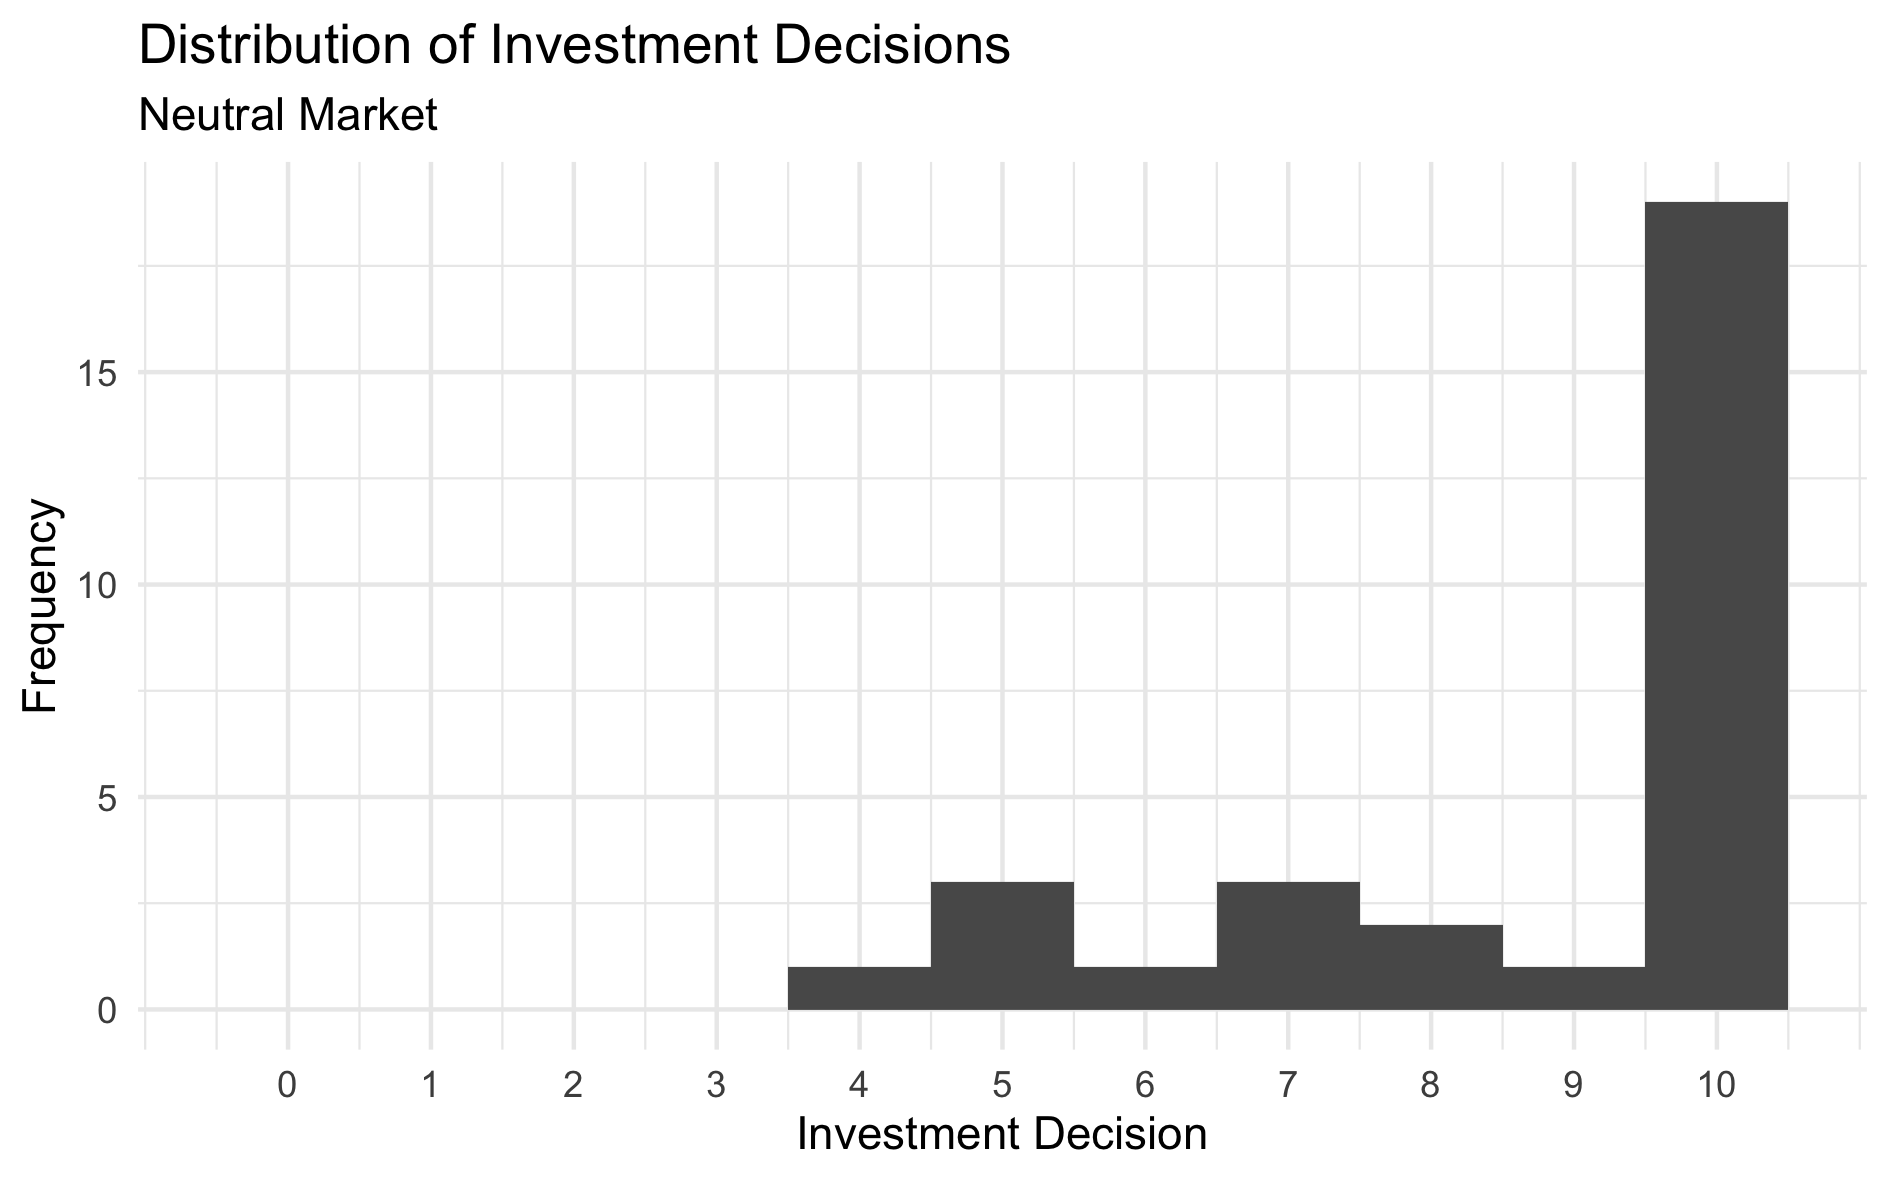
\includegraphics[width=0.7\textwidth]{investment-decisions-neutral-market-distribution}
\end{figure}

\begin{figure}[H]
	\centering
	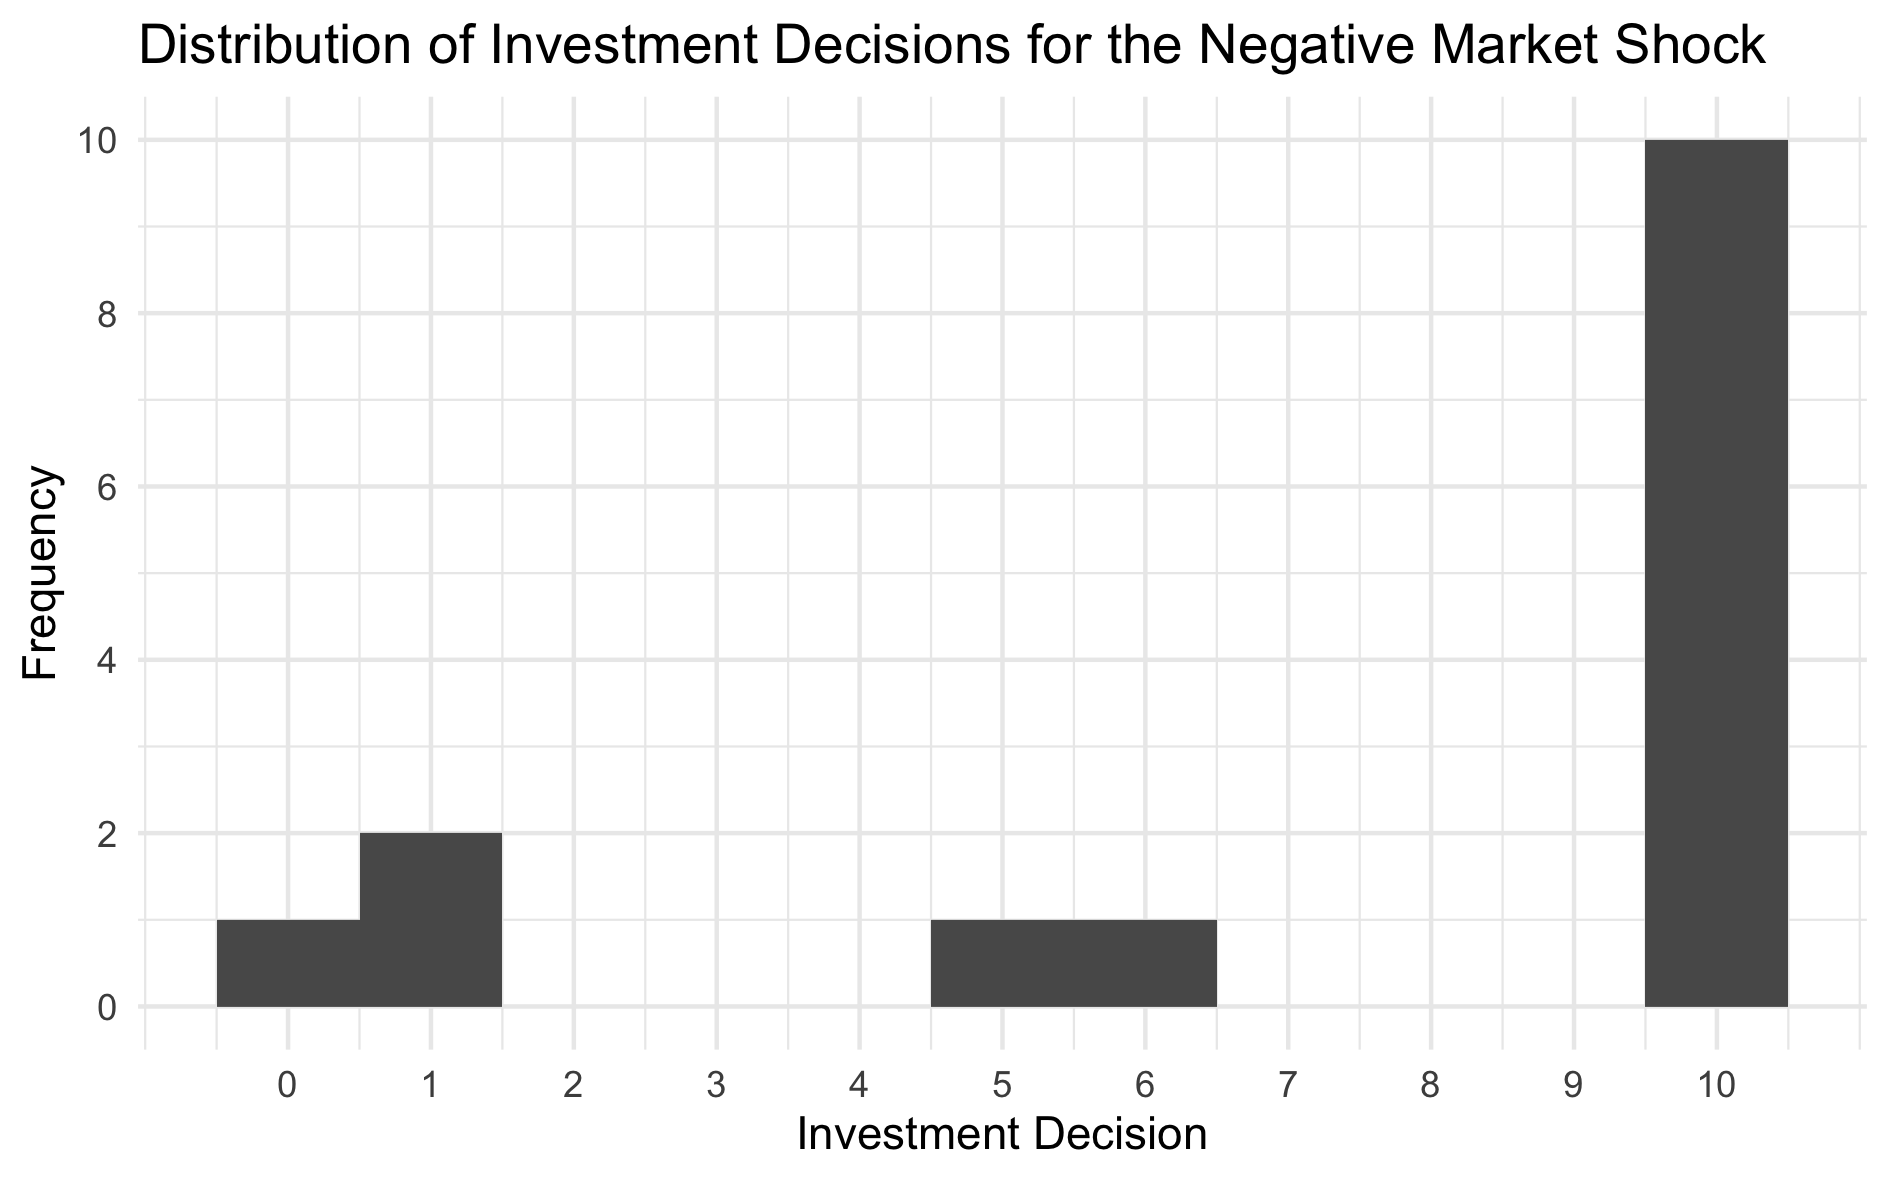
\includegraphics[width=0.7\textwidth]{investment-decisions-negative-shock-distribution}
\end{figure}

\begin{figure}[H]
	\centering
	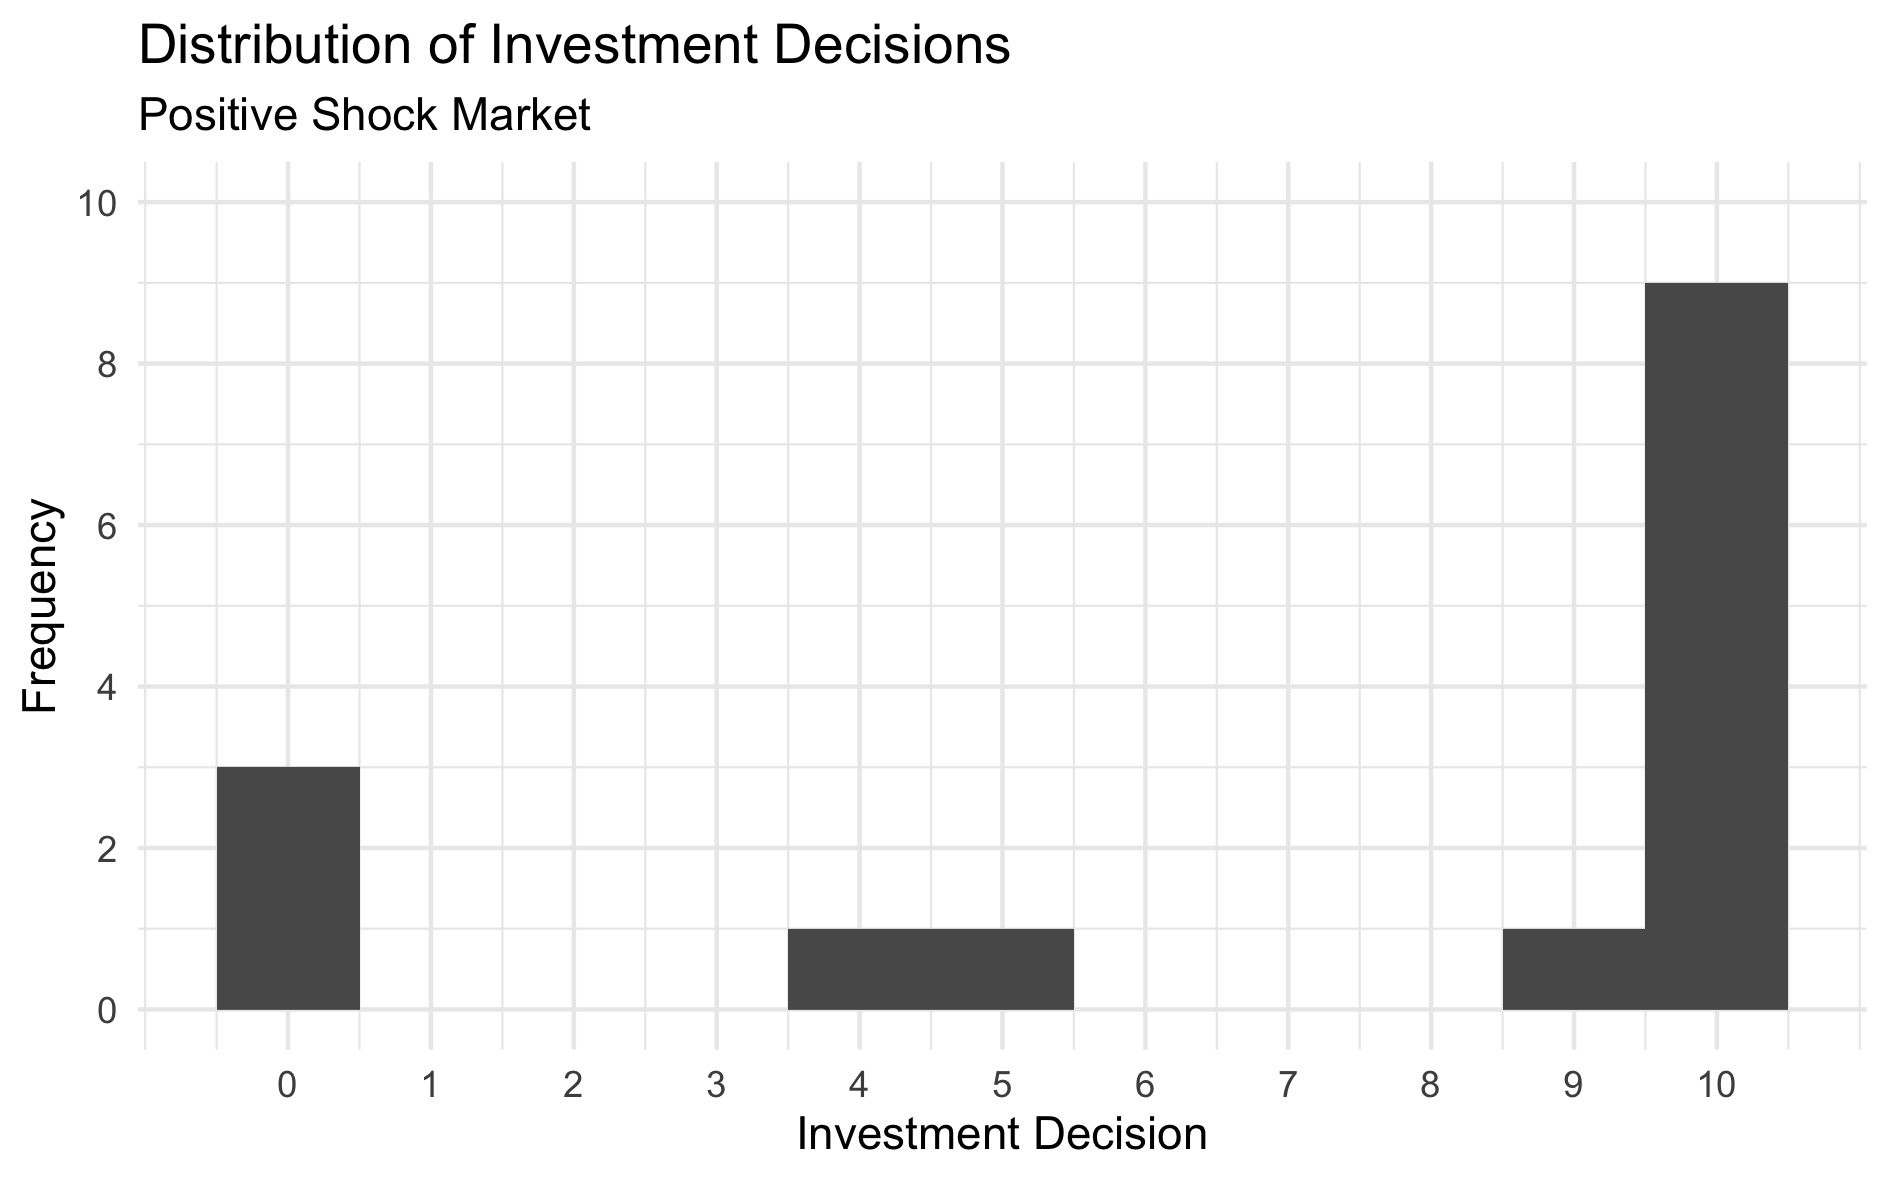
\includegraphics[width=0.7\textwidth]{investment-decisions-positive-shock-distribution}
\end{figure}

\begin{figure}[H]
	\centering
	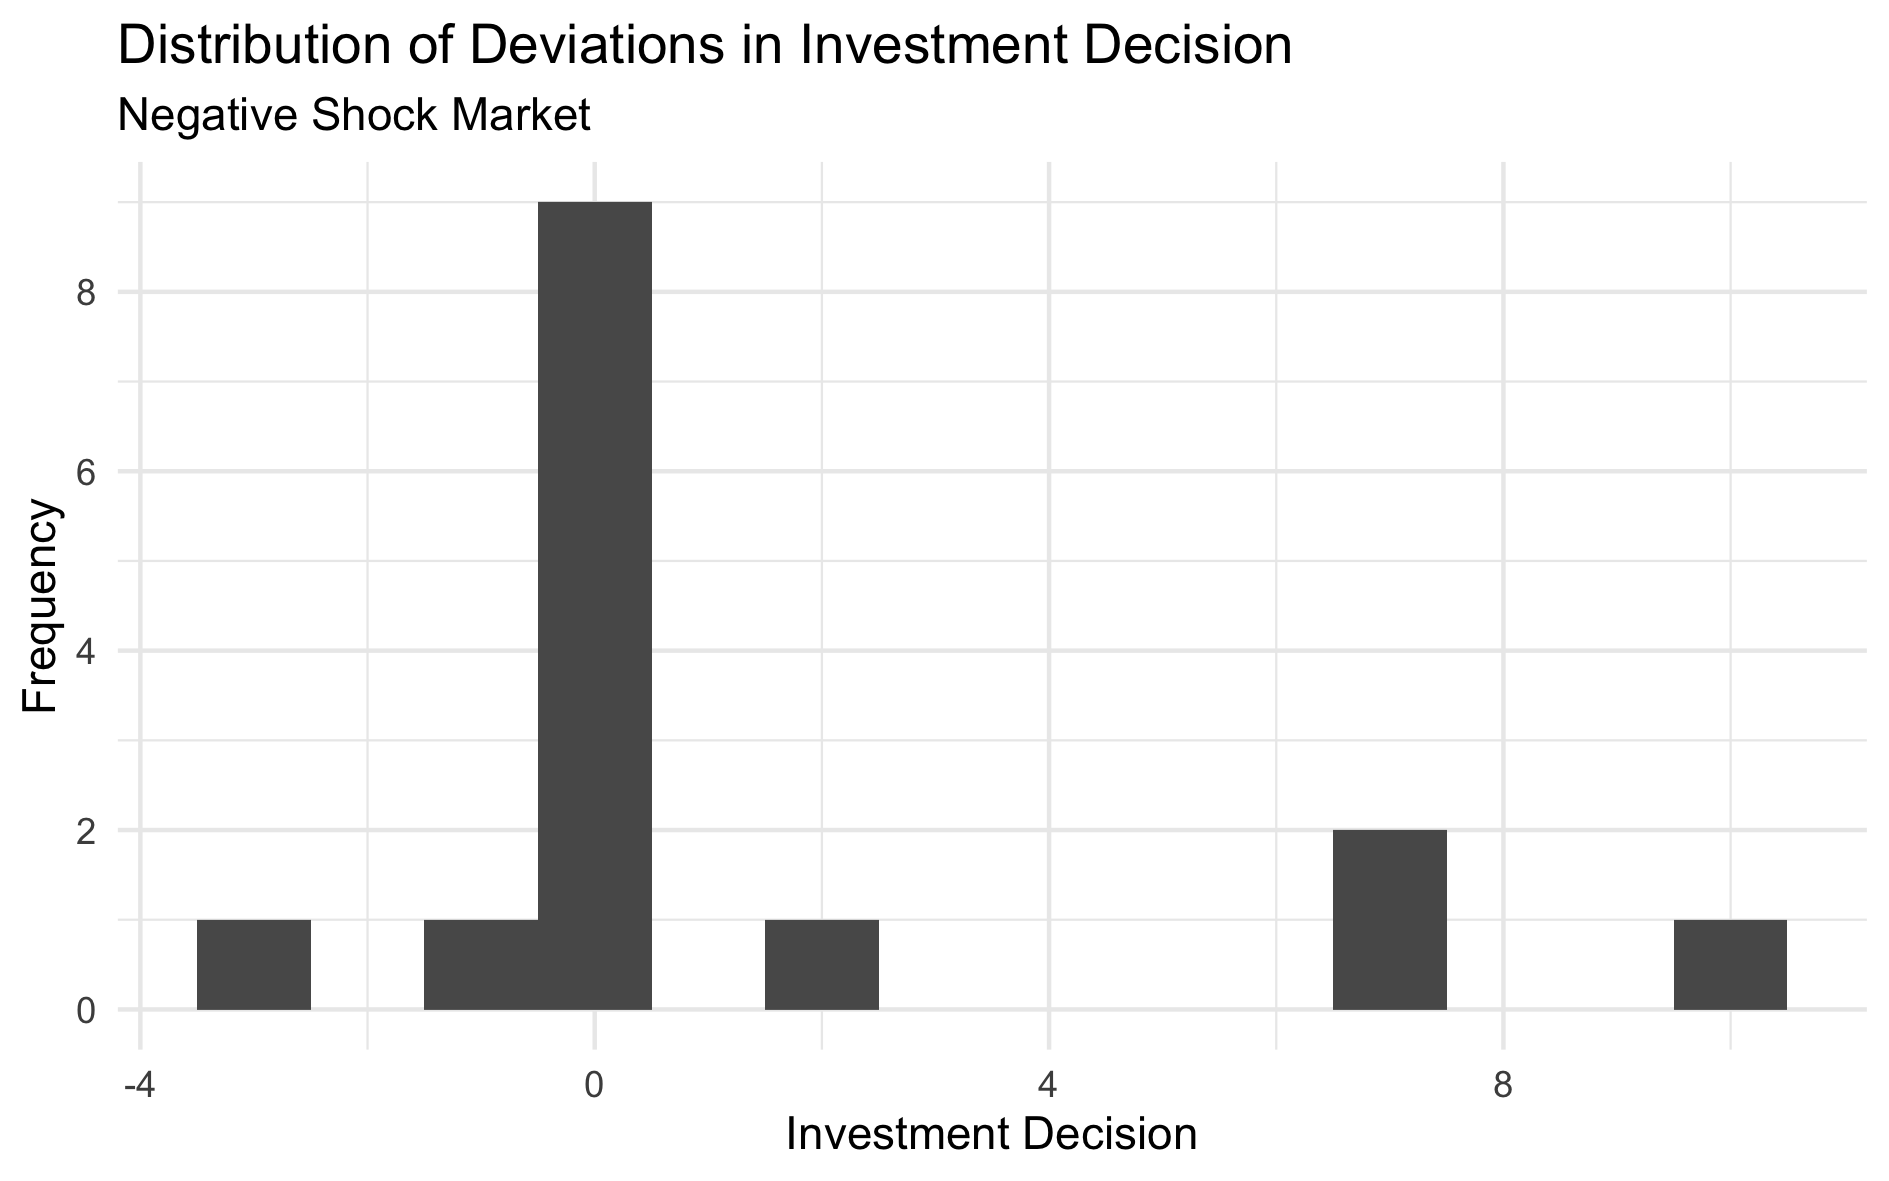
\includegraphics[width=0.7\textwidth]{investment-decision-deviations-negative-market-distribution}
\end{figure}

\begin{figure}[H]
	\centering
	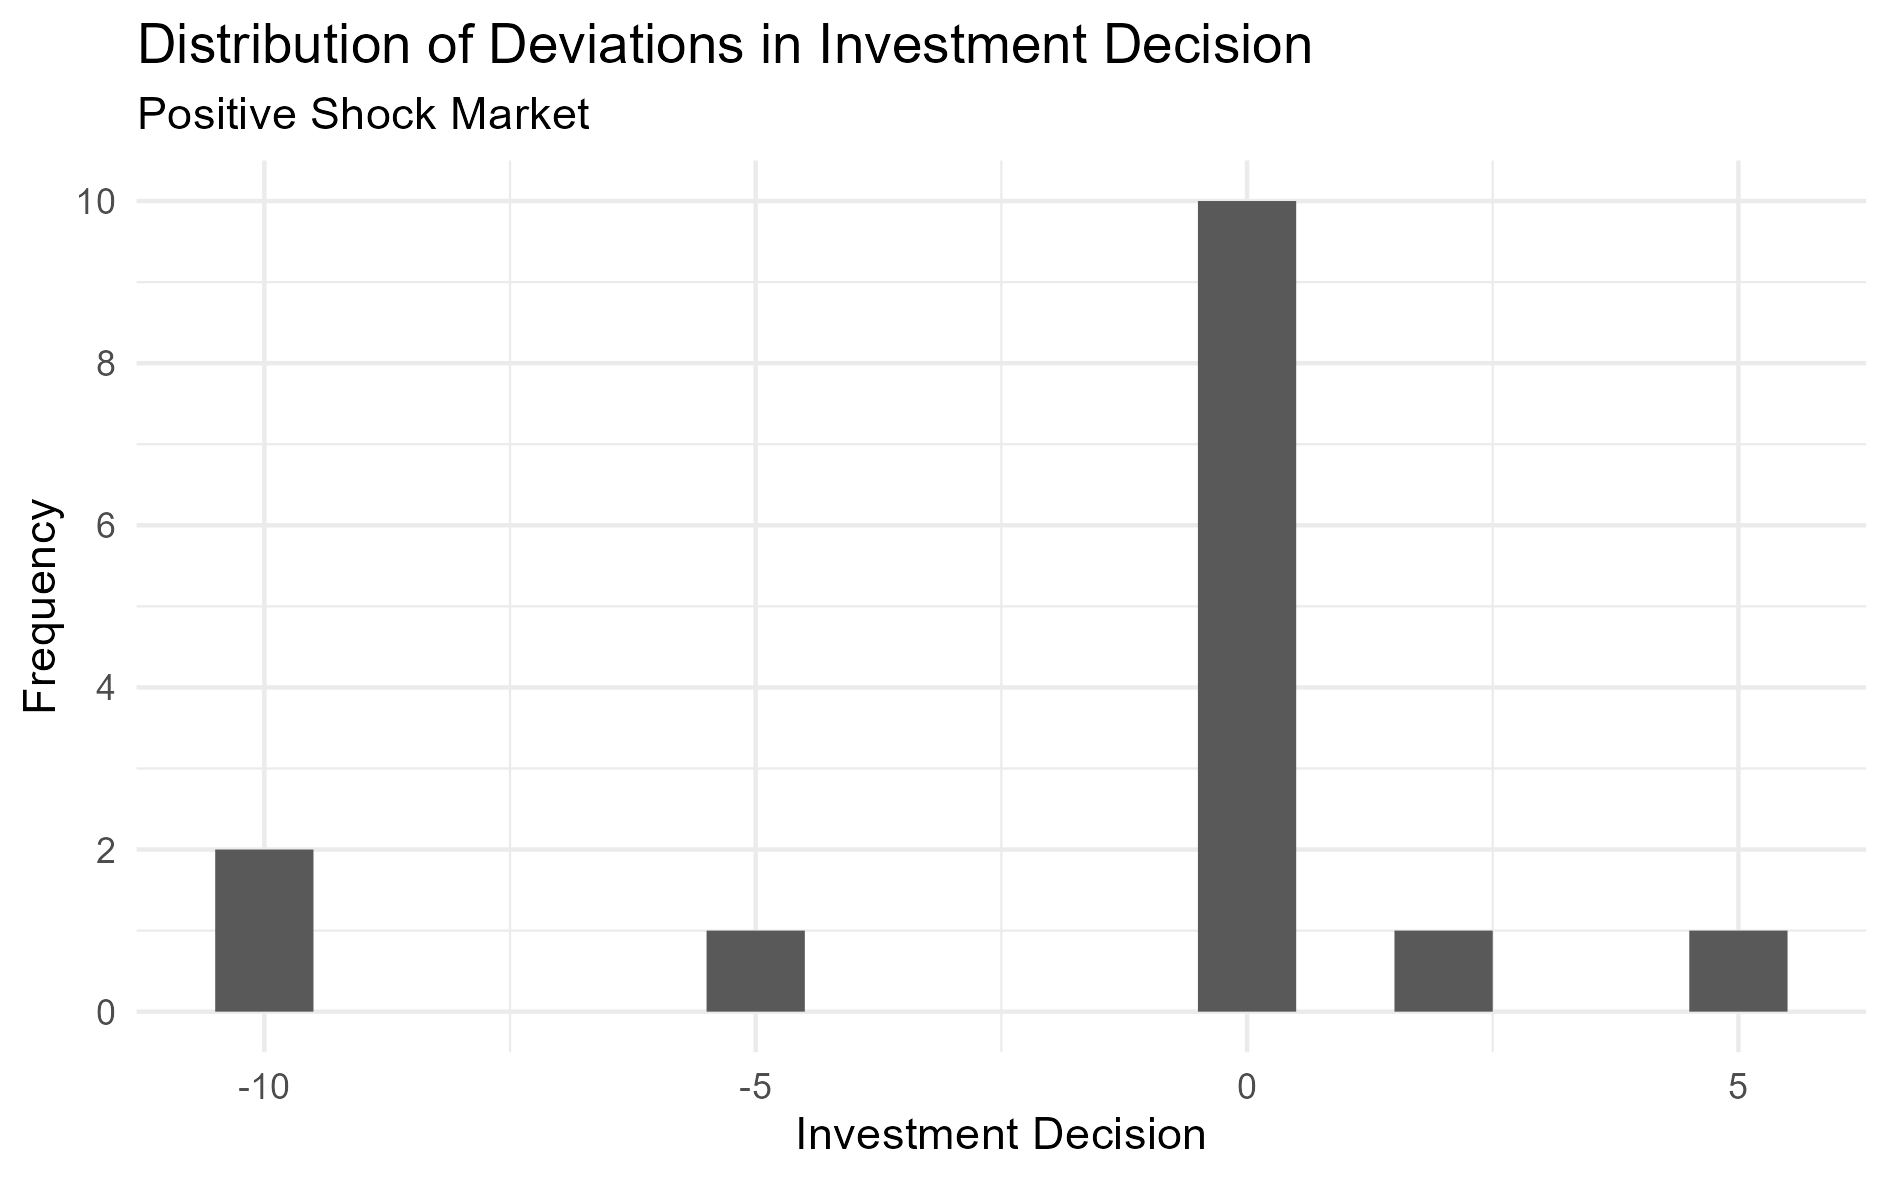
\includegraphics[width=0.7\textwidth]{investment-decision-deviations-positive-market-distribution}
\end{figure}


\section{Data Analysis}

\subsection{Difference in Differences Analyses}

A negative market shock decreases the mean investment decision by 0.26 (-0.26) euros and with that the average amount of money invested. A positive market shock increases the mean investment decision by 0.26 euros and with that the average amount of money invested.

A negative market shock increases the standard deviation by 0.72 euros and with that the variability in the investment decision distribution. A positive market shock decreases the standard deviation by 0.72 (-0.72) euros and with that the variability in the investment decision distribution.


\subsection{Mann-Whitney U Test}

\begin{nullhypothesis}
Individuals react symmetrically to positive and negative shocks. Thus, the deviation of the investment decision values in the neutral market state and the investment decision values in the shock market state are equal.
\end{nullhypothesis}

\begin{alternativehypothesis}
Individuals react asymmetrically to positive and negative shocks. Thus, deviation of the investment decision values in the neutral market state and the investment decision values in the shock market state are not equal.
\end{alternativehypothesis}

We fail to reject the null hypothesis since the $p\text{-value} = 0.2491 > p\text{-critical} = 0.05$ we fail to reject the null hypothesis. The change in the investment decisions following a positive market shock is not significantly different to the change in the investment decisions following a negative market shock.

\end{document}